\documentclass[border=6pt]{standalone}
\usepackage{tikz}
\begin{document}
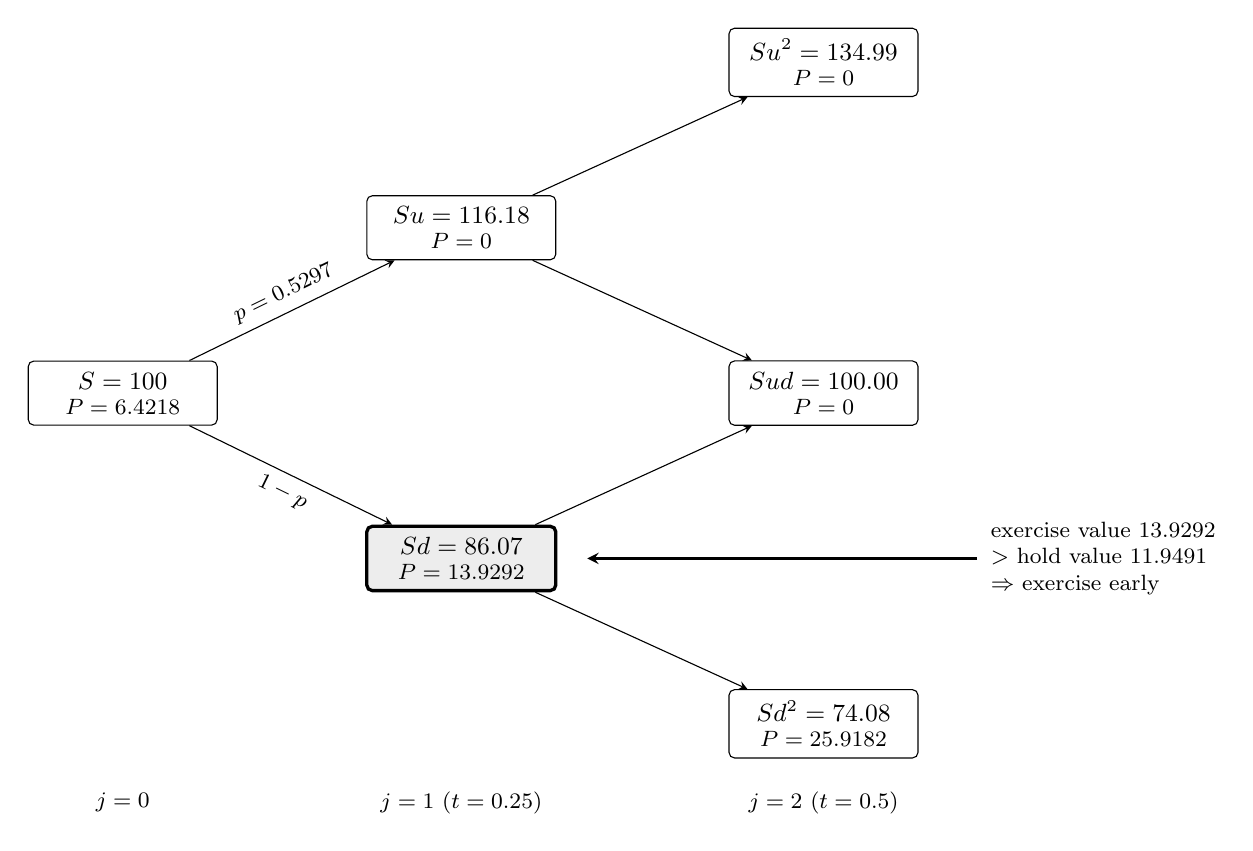
\begin{tikzpicture}[>=stealth,font=\small,
  nd/.style={draw,rounded corners=2pt,inner sep=4pt,minimum width=24mm,align=center},
  ex/.style={nd,very thick,fill=black!7}]
  \node[nd] (s)   at (0,0)      {$S=100$\\[-2pt]\footnotesize$P=6.4218$};
  \node[nd] (su)  at (4.3,2.1)  {$Su=116.18$\\[-2pt]\footnotesize$P=0$};
  \node[ex] (sd)  at (4.3,-2.1) {$Sd=86.07$\\[-2pt]\footnotesize$P=13.9292$};
  \node[nd] (suu) at (8.9,4.2)  {$Su^{2}=134.99$\\[-2pt]\footnotesize$P=0$};
  \node[nd] (sud) at (8.9,0)    {$Sud=100.00$\\[-2pt]\footnotesize$P=0$};
  \node[nd] (sdd) at (8.9,-4.2) {$Sd^{2}=74.08$\\[-2pt]\footnotesize$P=25.9182$};
  \draw[->] (s)  -- node[above,sloped,font=\footnotesize]{$p=0.5297$}(su);
  \draw[->] (s)  -- node[below,sloped,font=\footnotesize]{$1-p$}(sd);
  \draw[->] (su) -- (suu);  \draw[->] (su) -- (sud);
  \draw[->] (sd) -- (sud);  \draw[->] (sd) -- (sdd);
  \node[align=left,font=\footnotesize,anchor=west] at (10.9,-2.1)
    {exercise value $13.9292$\\ $>$ hold value $11.9491$\\ $\Rightarrow$ exercise early};
  \draw[->,thick] (10.85,-2.1) -- (5.9,-2.1);
  \node[font=\footnotesize] at (0,-5.2)   {$j=0$};
  \node[font=\footnotesize] at (4.3,-5.2) {$j=1$ ($t=0.25$)};
  \node[font=\footnotesize] at (8.9,-5.2) {$j=2$ ($t=0.5$)};
\end{tikzpicture}
\end{document}
